\documentclass[a4paper]{article}

% Packages.
\usepackage{amsmath}
\usepackage{amsthm}
\usepackage[answerdelayed]{exercise}
\usepackage[usenames,dvipsnames]{color}

% Definitions.
\theoremstyle{definition}
\newtheorem{definition}{Definition}

\renewcommand{\ExerciseHeader}{\vspace{7mm}\par\noindent\textbf{\large
\ExerciseName\ \ExerciseHeaderNB\ExerciseHeaderTitle
\ExerciseHeaderOrigin}\par}

\renewcommand{\AnswerHeader}{\par\noindent\textbf{
Answer of \ExerciseName\ \ExerciseHeaderNB}\par}

% Options.


\title{The correlation}
\author{Guillaume Filion}
\usepackage{Sweave}
\begin{document}
\maketitle


%% The problem %%
\section{The problem}

In 1997, Robert Clarke and collaborators conducted a meta-analysis to
determine the quantitative importance of dietary fatty acids to blood
concentrations of cholesterol. They report 6 studies with the same protocol
applied to 14 subjects each. Here is their data (the study is real but
the data is fake):

\begin{center}
  \par
  \begin{tabular}{ccc}
    Saturated fat in diet & Blood cholesterol \\
    \% total calories     & mmol/L \\
    \hline
    25.7 & 5.9 \\
    5.1 & 5.9 \\
    13.0 & 4.8 \\
    20.5 & 5.8 \\
    7.0 & 6.3 \\
    27.9 & 6.1
  \end{tabular}
\end{center}

In your \texttt{R} session, manually enter the data in 2 vectors of
length 6 (\texttt{diet}, \texttt{blood}).

\begin{Schunk}
\begin{Sinput}
> diet <- c(25.7, 5.1, 13.0, 20.5, 7.0, 27.9);
> blood <- c(5.9, 5.9, 4.8, 5.8, 6.3, 6.1);
\end{Sinput}
\end{Schunk}

\begin{Exercise}
Can we assume that the data is Gaussian? If not, can we assume that the
response variable (blood cholesterol) is Gaussian given the diet?
What is the null hypothesis?
\end{Exercise}
\begin{Answer}
We can assume that given a certain diet, the distribution of blood
cholesterol is Gaussian (`reaction norms' are often Gaussian).
Like for the $t$ test, the null hypothesis can be formulated as follows:
\begin{enumerate}
\item
The blood cholesterol is sampled from a Gaussian distribution.
\item
\label{reject}
The parameters are unknown, but equal in all cases.
\item
Sampling is IID.
\end{enumerate}
\end{Answer}

\begin{Exercise}
We would like to find a statistic that measures `association' between
the two variables. Can you suggest a score? What is the alternative
hypothesis?
\end{Exercise}
\begin{Answer}
The coefficient of correlation $r$ is a good score for the problem at
hand. By definition it is the covariance of the two variables divided
by he product of their standard deviations.

\begin{equation*}
r = \frac{\sum_{i=1}^6(x_i - \bar{x})(y_i - \bar{y})}
  {\sqrt{\sum_{i=1}^6(x_i - \bar{x})^2 \sum_{i=1}^6(y_i - \bar{y})^2}}.
\end{equation*}

You can check that this is the same as computing the covariance
(\texttt{cov}) between two vectors and dividing by the product of their
standard deviations (\texttt{sd}). The $n-1$ terms cancel out in the
numerator and the denominator.

In the alternative hypothesis, item \ref{reject} is replaced by `The
expected value of the response variable is a linear function of the
independent variable (the diet here)'.
\end{Answer}


%% The test statistic %%
\section{The test statistic}

For this problem, \texttt{R} made our life particulary easy with the
function \texttt{cor} which computes just our test statistic $r$.

\begin{Exercise}
Plot the data in the $(x,y)$ plane. Add the regression line with
\texttt{abline(lm(blood \~\ diet))}. Display the coefficients of
the line by calling \texttt{lm(blood \~\ diet)}. Also compute
\texttt{cor(blood, diet) * sd(blood) / sd(diet)}, what do you observe?
\end{Exercise}
\begin{Answer}
\begin{Schunk}
\begin{Sinput}
> plot(diet, blood);
> abline(lm(blood ~ diet), col=2);
> lm(blood ~ diet);
\end{Sinput}
\begin{Soutput}
Call:
lm(formula = blood ~ diet)

Coefficients:
(Intercept)         diet  
   5.730375     0.004211  
\end{Soutput}
\begin{Sinput}
> cor(blood, diet)*sd(blood)/sd(diet);
\end{Sinput}
\begin{Soutput}
[1] 0.004211178
\end{Soutput}
\end{Schunk}
\includegraphics{correlation-002}
\par
The last term is the slope of the line. This is a property of the
regression line, the slope is intimately linked to the correlation
(by the formula used above).
\end{Answer}

\begin{Exercise}
Verify by the formula, or with some examples at the terminal that $r$
is invariant by translation and scaling \textbf{of any or both of the
variables}. What does that mean for the resampling of $r$?
\end{Exercise}
\begin{Answer}
The proof is similar to that used for the effect size $t$. To verify
it you can try different transformations.
\begin{Schunk}
\begin{Sinput}
> r.obs <- cor(blood, diet);
> r.obs;
\end{Sinput}
\begin{Soutput}
[1] 0.07770512
\end{Soutput}
\begin{Sinput}
> cor(blood+1, diet);
\end{Sinput}
\begin{Soutput}
[1] 0.07770512
\end{Soutput}
\begin{Sinput}
> cor(pi*blood+1, diet);
\end{Sinput}
\begin{Soutput}
[1] 0.07770512
\end{Soutput}
\begin{Sinput}
> cor(pi*blood+1, diet+2);
\end{Sinput}
\begin{Soutput}
[1] 0.07770512
\end{Soutput}
\begin{Sinput}
> cor(pi*blood+1, -1*diet+2);
\end{Sinput}
\begin{Soutput}
[1] -0.07770512
\end{Soutput}
\end{Schunk}
\par
Note that the correlation changes sign but not value when one variable
is multiplied by a negative number.

This means that we can resample $r$ from standard Gaussian variables
because all Gaussian variables have the same distribution of $r$ under
the null hypothesis.
\end{Answer}

\begin{Exercise}
Resample $r$, finish the test, estimate the p-value, compare with the
results of \texttt{cor.test}.
\end{Exercise}
\begin{Answer}
\begin{Schunk}
\begin{Sinput}
> r.smpl <- rep(NA, 10000);
> for (i in 1:10000) {
+   r.smpl[i] <- cor(rnorm(6), diet);
+ }
> plot(density(r.smpl), main="Density of r", xlab="Value");
> abline(v=r.obs, col=2);
> quantile(abs(r.smpl), probs=0.95);
\end{Sinput}
\begin{Soutput}
      95% 
0.8178391 
\end{Soutput}
\begin{Sinput}
> mean(abs(r.smpl) > r.obs);
\end{Sinput}
\begin{Soutput}
[1] 0.8826
\end{Soutput}
\begin{Sinput}
> cor.test(blood, diet);
\end{Sinput}
\begin{Soutput}
	Pearson's product-moment correlation

data:  blood and diet 
t = 0.1559, df = 4, p-value = 0.8837
alternative hypothesis: true correlation is not equal to 0 
95 percent confidence interval:
 -0.7832498  0.8365138 
sample estimates:
       cor 
0.07770512 
\end{Soutput}
\end{Schunk}
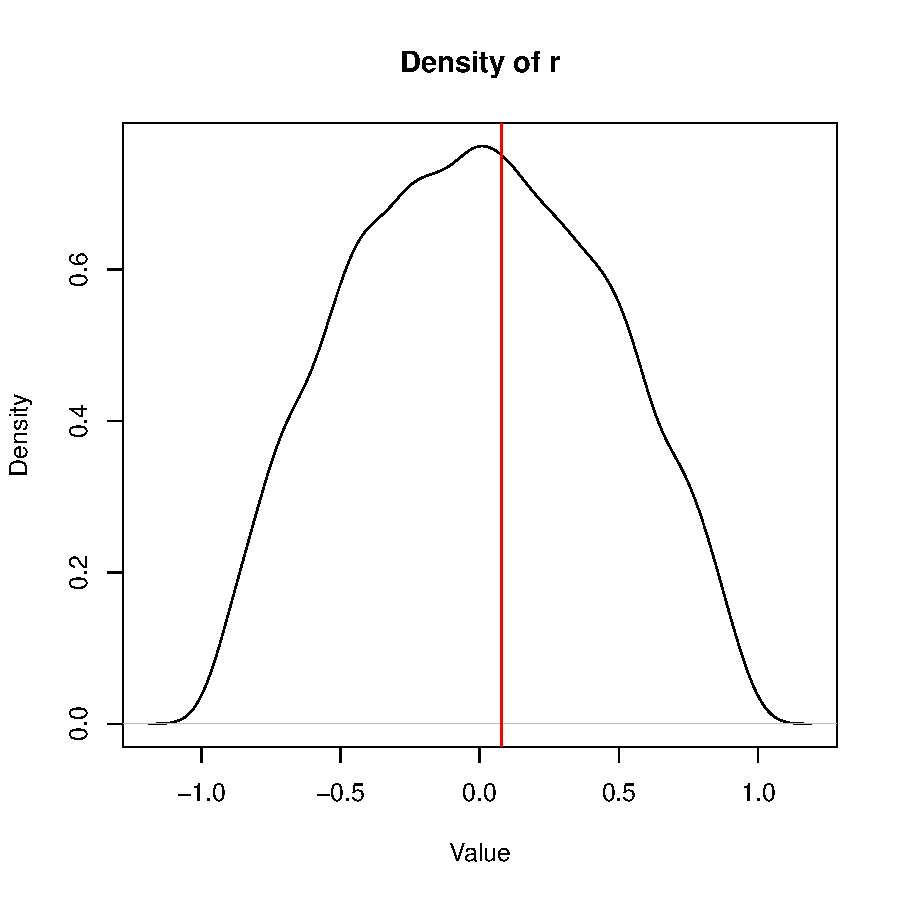
\includegraphics{correlation-004}
\end{Answer}

%% Properties of the correlation %%
\section{Properties of the correlation}

The coefficient of correlation has a few properties worth mentioning,
mostly because \textbf{they can be very dangerous}.

\begin{Exercise}
What is the maximum value that the coefficient of correlation can take?
What is the minimum?
\end{Exercise}
\begin{Answer}
The coefficient of correlation is always between -1 and 1 (for real
variables). This is a direct result of the Cauchy-Schwarz inequality,
but it is rather difficult to prove if you don't know this result.
You can verify by yourself by trying different inputs to
\texttt{cor}. The highest you can find will be for
\texttt{cor(blood, blood)} and the lowest for \texttt{cor(blood, -blood)}.
\end{Answer}

\begin{Exercise}
What does that mean if two variables have a coefficient of correlation of
1 in absolute value?
\end{Exercise}
\begin{Answer}
This means that one of the variables is a linear transformation of the
other, \textit{i.e.} a scaling and translation of the other. You can see
it with \texttt{cor(blood, 3*blood+4)} etc.
\end{Answer}

\begin{Exercise}
What does that mean if two variables have a coefficient of correlation of
0? Assign to \texttt{x} all the integer numbers between -5 and 5. Specify
\texttt{y <- x\^{}2}, plot the variables in the $(x,y)$ plane and compute their
correlation. Conclude.
\end{Exercise}
\begin{Answer}
\begin{Schunk}
\begin{Sinput}
> x <- -5:5;
> y <- x^2;
> plot(x,y);
> cor(x,y);
\end{Sinput}
\begin{Soutput}
[1] 0
\end{Soutput}
\end{Schunk}
\includegraphics{correlation-005}
\par
The coefficient of correlation is sometimes called the coefficient of
\textbf{linear} correlation because it measures only linear trends between
two variables. The coefficient of correlation should \textbf{never} be
interpreted without a plot of $y$ versus $x$, because many variables show
a strong mutual dependency, but no linear correlation.
\end{Answer}


\cleardoublepage
\shipoutAnswer
\end{document}

